\begin{figure}
    \centering
    \begin{subfigure}[b]{0.3\textwidth}
         \centering
         \caption{}
         % \includesvg[pretex=\tiny, width=\textwidth]{../Figures/working/F1_ParadigmPredictions/chromaticity231109.svg}
         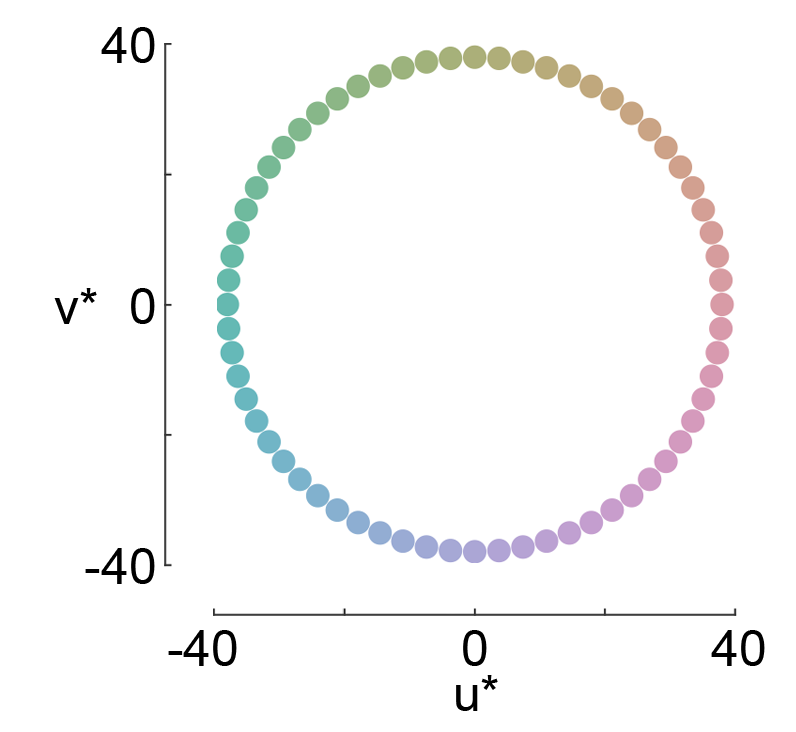
\includegraphics[width=\textwidth]{../Figures/working/F1_ParadigmPredictions/a.png}
         \label{fig:StimuliChromaticities}
    \end{subfigure}
    \hfill
    \begin{subfigure}[b]{0.65\textwidth}
         \centering
         \caption{}
         % \includesvg[pretex=\tiny, width=\textwidth]{../Figures/working/F1_ParadigmPredictions/epochs230620.svg}
        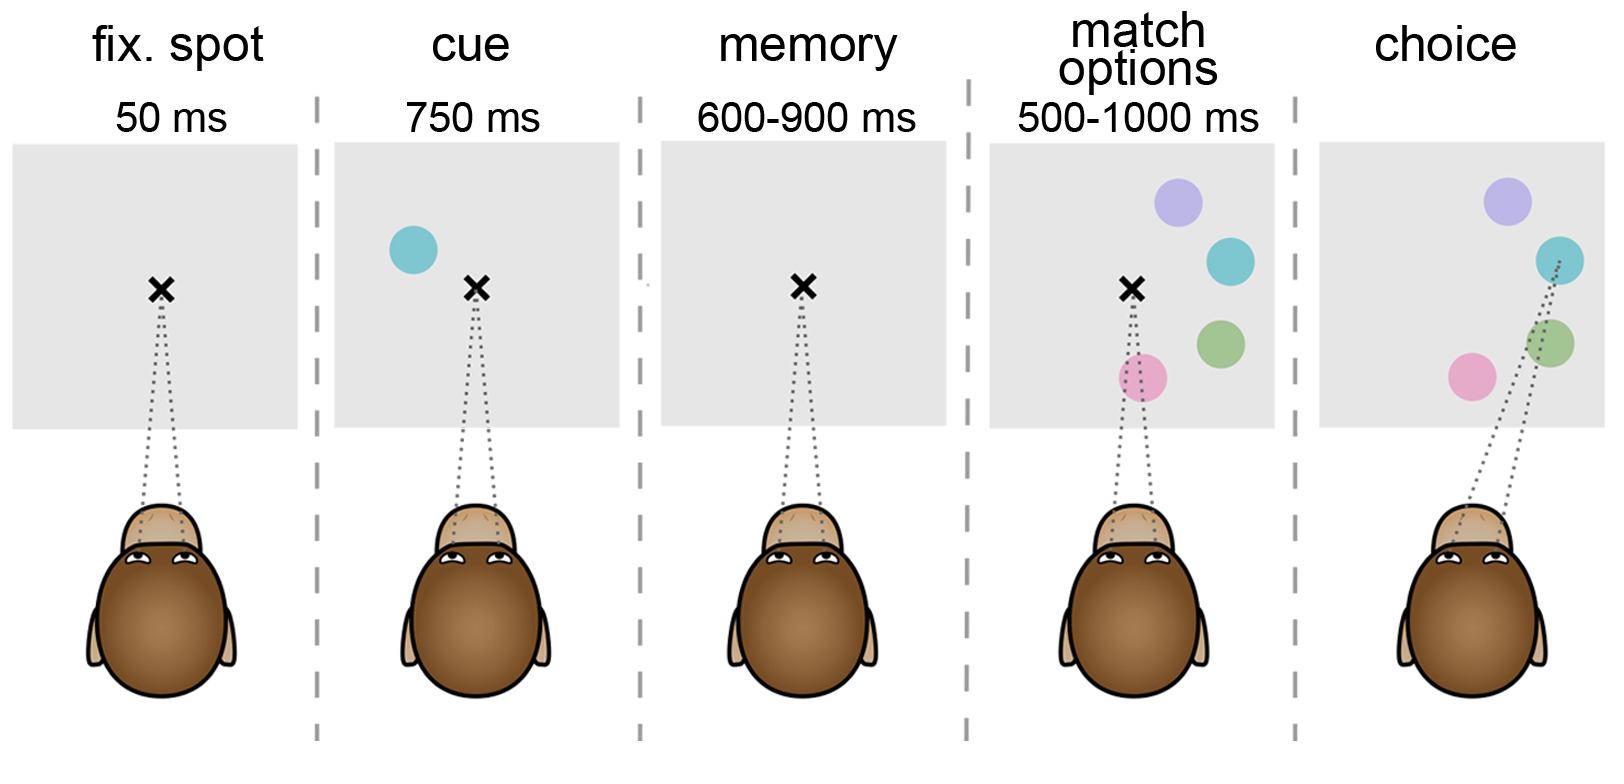
\includegraphics[width=\textwidth]{../Figures/working/F1_ParadigmPredictions/b.png}
         \label{fig:epochs}
    \end{subfigure}

    \begin{subfigure}[b]{0.45\textwidth}
         \centering
         \caption{}
         % \includesvg[pretex=\tiny, width=\textwidth]{../Figures/working/F1_ParadigmPredictions/bias1-230620.svg}
        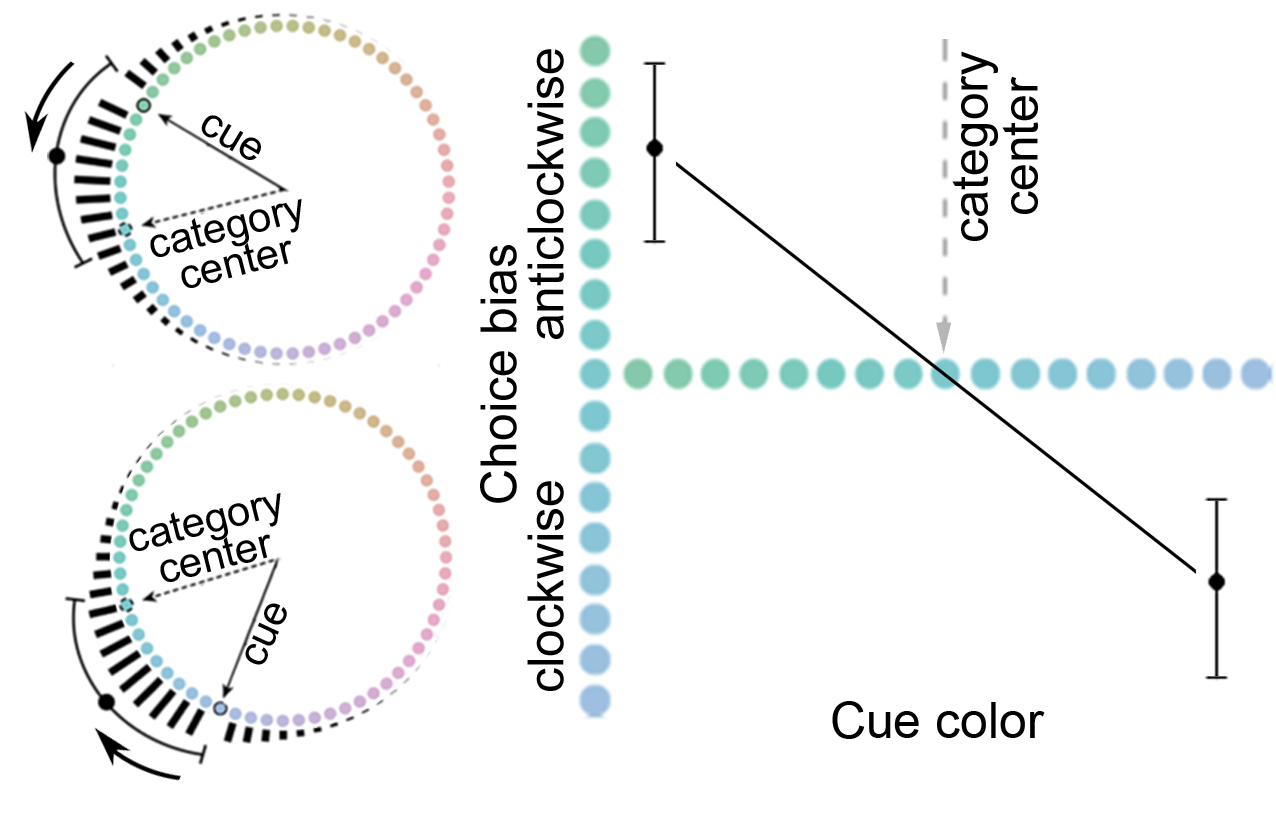
\includegraphics[width=\textwidth]{../Figures/working/F1_ParadigmPredictions/c.png}
         \label{fig:Bias1}
    \end{subfigure}
    %     \hfill
    % \begin{subfigure}[b]{0.20\textwidth}
    %      \centering
    %      \caption{}
    %      % \includesvg[pretex=\tiny, width=\textwidth]{../Figures/working/F1_ParadigmPredictions/bias2-230620.svg}

    %      \label{fig:Bias2}
    % \end{subfigure}
    % \hfill
    % \begin{subfigure}[b]{0.20\textwidth}
    %      \centering
    %      \caption{}
    %      \includegraphics[width=\textwidth]{example-image-a}
    %      \label{fig:BiasLinear}
    % \end{subfigure}
    \hfill
    \begin{subfigure}[b]{0.45\textwidth}
         \centering
         \caption{}
         % \includegraphics[width=\textwidth]{example-image-a}
        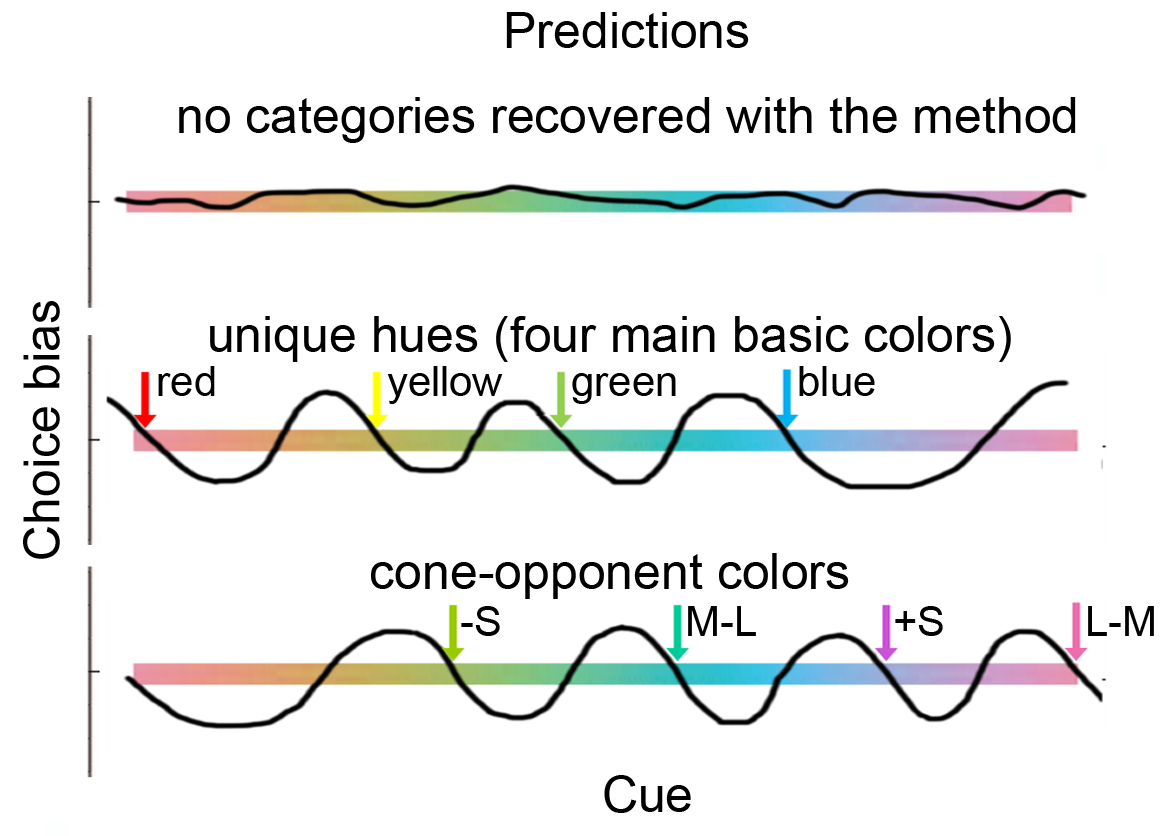
\includegraphics[width=\textwidth]{../Figures/working/F1_ParadigmPredictions/d.png}
         \label{fig:BiasPredictions}
    \end{subfigure}

    % 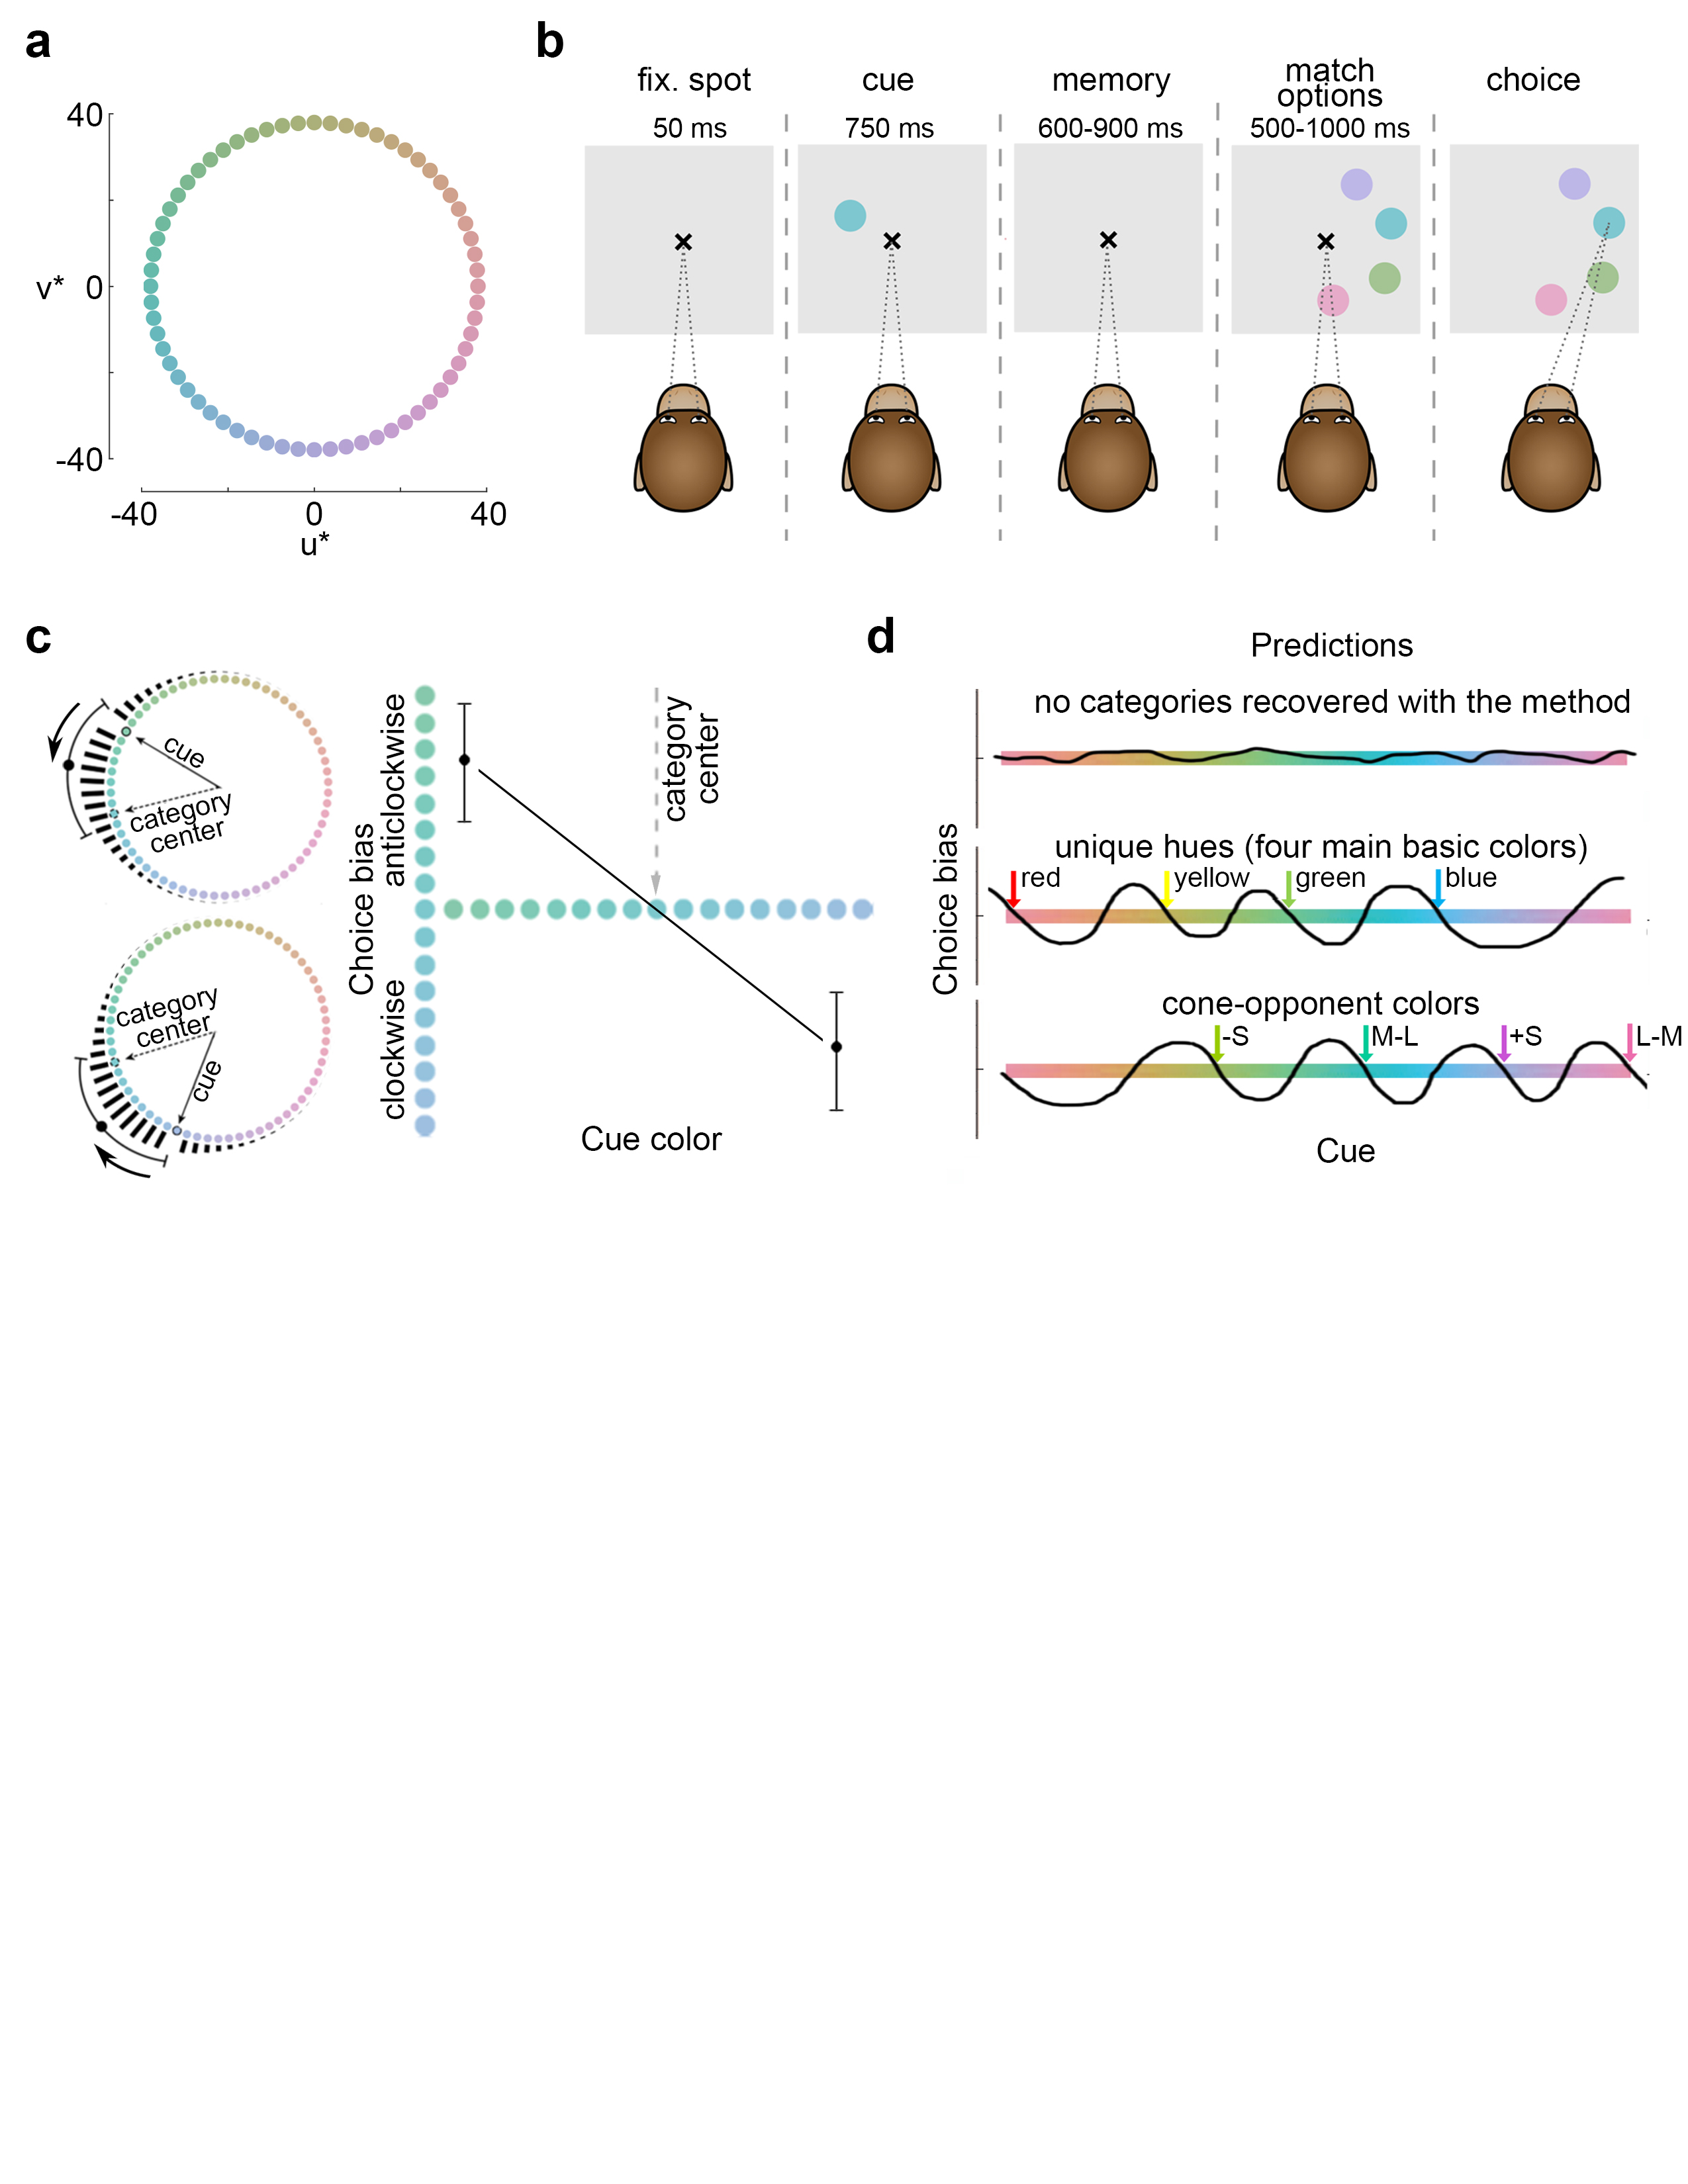
\includegraphics[width=\textwidth,trim={0 12cm 0 0},clip]{../Figures/flat/F1_ParadigmPredictions_3.jpg}
    
    \caption{\textbf{4-Alternative Forced Choice (4-AFC), Delayed Match to Sample Paradigm.}
    \emph{A.} Cue and choice colors in the $u^*v^*$ plane of CIELUV. Colors were defined to be equi-luminant and equi-saturated in CIELUV.
    \emph{B.} The epochs of the paradigm: a trial is initiated when fixation upon a fixation cross is maintained for 50ms. Following this a cue color is shown. This disappears and the animal must remember this color. 4 options appear on the screen, with 1 being a direct match to the cue. Once the fixation cross disappears, the monkey is allowed to make a choice by looking at the their choice, and they are rewarded if they select the choice which matches the cue for that trial.
    \emph{C.} The presence of color categories can cause bias. This bias will be in the direction of the category center.
    Where the magnitude of bias crosses zero from anticlockwise to clockwise bias, we label this as the center of the category.
    \emph{D.} Competing hypotheses for the structure of biases, based on existing theories.
} 
    \label{fig:ParadigmAnalysisPredictions}
    
\end{figure}

Color categories are identified by color terms, of which the Basic Color Terms are considered prominent \citep{berlin_basic_1969}.
One hypothesis is that among the BCTs, red, green, blue, and yellow are universal \citep{heider_universals_1972,regier_focal_2005}
and endowed by hard-wired neural mechanisms present at birth \citep{bornstein_categories_1976,lindsey_universality_2006}. 
This idea, put forth 150 years ago \citep{hering_zur_1875}, predicts observed cross-cultural color naming patterns \citep{jameson_evolutionary_2009,baronchelli_modeling_2010,lindsey_hunter-gatherer_2015,abbott_focal_2016}
and is consistent with some neurophysiological results \citep{clifford_electrophysiological_2009,holmes_neurophysiological_2009,brouwer_categorical_2013,bird_categorical_2014,yang_cortical_2016,forder_colour_2017}
. 
Behavioral work in infants provides perhaps the strongest evidence for a biological origin of color categories \citep{franklin_new_2004,ozturk_language_2013}; this work suggests that the innate categories may be defined by retinal cone-opponent mechanisms rather than basic colors \citep{skelton_biological_2017,maule_color_2019}.
Another hypothesis is that color categories emerge in development, instructed by language and culture \citep{roberson_color_2005, regier_language_2009, cibelli_sapir-whorf_2016}, and possibly involving an interplay of innate and developmental factors \citep{kay_language_2006,franklin_lateralization_2008,regier_language_2009}. 
This hypothesis is promoted by variability in color naming patterns across languages and individuals \citep{davidoff_colour_1999,roberson_color_2000,paramei_online_2018,webster_variations_2002}.
Current consensus is that some aspect of adult color category behavior is acquired through experience; but the extent to which the origin of color categories is innate remains unresolved \citep{davidoff_nature_2009,skelton_colour_2023}.

One approach to the origin of color categories that sidesteps difficulties working with human infants is studies of trichromatic non-human primates. 
The few studies on this topic have come to different conclusions: one found color categories in macaques consistent with categories in human adults \citep{sandell_color_1979}; one tested for a blue-green category boundary and found it in humans but not in baboons \citep{fagot_cross-species_2006}; and one found different categories in the two macaques tested, apparently dependent on the animals’ experiences \citep{panichello_error-correcting_2019}.

\paragraph{Measuring color categories in macaque monkeys}

Addressing the question of color categories in monkeys requires overcoming several challenges. 
First, how to measure color categories without teaching the animals the categories \citep{essock_color_1977,matsuno_color_2004}.
Second, how to specify the color stimuli \citep{siuda-krzywicka_biological_2019}; for example, specifying the colors as wavelengths \citep{sandell_color_1979}
is not appropriate \citep{davidoff_cross-species_2010}. 
Third, how to obtain precise data across the full circle of hues. 
A match-to-sample paradigm using colors defined in a perceptually uniform color space (\autoref{fig:StimuliChromaticities}) provides a potential solution \citep{bae_why_2015,panichello_error-correcting_2019}.
But to test for consistent color categories across animals, we need not only to ensure precision in the matched colors but also to avoid the possibility of reinforcing biases acquired while the animals perform the task. 
So, rather than having animals match a cued color to a spot on a continuous ring of colors and occasionally rewarding them for inaccurate matches as in the established paradigm, we adapted it into an alternative-forced-choice task in which a direct match to the cue was available in every trial and the monkeys were only rewarded for making the direct match (\autoref{fig:epochs}). 
One consequence of the adapted paradigm is that it requires considerable data to satisfactorily sample category performance across the space of colors. 
Four animals performed the task, completing at total of 299,690 trials over 232 sessions (\autoref{fig:Indi_difficulty}).

\begin{figure}
    \centering
        \begin{subfigure}[t]{0.36\textwidth}
         \centering
         \caption{}
         \includesvg[pretex=\ttiny,width=\textwidth]{../Figures/working/F2_CombinedMMResults/difficulty_combinedData231110-004913.svg}
         \label{fig:CombinedDifficulty}
    \end{subfigure}
    \hfill
    \begin{subfigure}[t]{0.36\textwidth}
         \centering
         \caption{}
         \includesvg[pretex=\ttiny, width=\textwidth]{../Figures/working/F2_CombinedMMResults/F2_CombinedMMResults_fromModelOutput_MixMod_linear_231110-001902.svg}
         \label{fig:CombinedLinear}
    \end{subfigure}
    \hfill
    \begin{subfigure}[t]{0.25\textwidth}
         \centering
         \caption{}
         \includesvg[pretex=\ttiny, width=\textwidth]{../Figures/working/F2_CombinedMMResults/F2_CombinedMMResults_fromModelOutput_MixMod_polar_231110-001903.svg}
         \label{fig:CombinedPolar}
    \end{subfigure}
    \caption{\textbf{Bias as a function of hue, for data collapsed over 4 animals.} 
    }
    \label{fig:AvResults}
\end{figure}

If a monkey has a color category, the category will be captured by the zero-crossing of the negative slope in a plot of the choice bias (\autoref{fig:Bias1}%/Bias2/BiasLinear
). 
The approach is data-driven so it will recover whatever categories exist; nonetheless, before collecting the data we considered three possibilities. 
First, that the monkeys would show no color categories, as predicted by the work in baboons \citep{davidoff_cross-species_2010}
(\autoref{fig:BiasPredictions}, top);
second, that macaque color categories would correspond to the four main basic color categories, consistent with data in human adults \citep{bae_why_2015}
(\autoref{fig:BiasPredictions}, middle); and third, that macaque color categories would align with the cone-opponent mechanisms predicted by data in human infants \citep{skelton_biological_2017}
(\autoref{fig:BiasPredictions}, bottom). 
The animals performed well on the task, showing an average lapse rate on the easiest trials of 9\% (\autoref{fig:CombinedDifficulty}; plots of individual animals in \autoref{fig:Indi_difficulty}) and providing clear evidence of choice biases (\autoref{fig:AvResults}).
But the recovered color categories analyzed with a mixture model do not support any of the predictions. 
Instead, the animals appeared to show two consensus color categories. 
These categories are not obviously aligned with either of the cone-opponent mechanisms (arrowheads, \autoref{fig:CombinedPolar}) but could instead be described as “warm” and “cool” (teal-colored and salmon-colored radiating wedges in \autoref{fig:CombinedPolar}; data for individual animals is shown in \autoref{fig:BiasCurvesIndividual}).

\paragraph{Two possible explanations for choice biases in macaque monkeys}

\begin{figure}
    \centering

    \begin{subfigure}[b]{0.3\textwidth}
         \centering
         \caption{}
         \includegraphics[width=\textwidth]{example-image-a}
         \label{fig:TCCCartoonA}
    \end{subfigure}
    \begin{subfigure}[b]{0.3\textwidth}
         \centering
         \caption{}
         \includegraphics[width=\textwidth]{example-image-a}
         \label{fig:TCCCartoonB}
    \end{subfigure}
    
    \begin{subfigure}[b]{0.3\textwidth}
         \centering
         \caption{}
        \includesvg[pretex=\tiny, width=\textwidth]{../Figures/working/F3_TCCModel/F3_TCCModel_og_Output_fromPreProcessedData_postCombined_MixMod_polar_231110-022720.svg}
         \label{fig:TCCModel_og}
    \end{subfigure}
    \begin{subfigure}[b]{0.3\textwidth}
         \centering
         \caption{}
         \includesvg[pretex=\tiny, width=\textwidth]{../Figures/working/F3_TCCModel/TCCDemo_ssnu_fromModelOutput_MixMod_polar_231110-022647.svg}
         \label{fig:TCCModel_ssnu}
    \end{subfigure}

    \begin{subfigure}[b]{0.3\textwidth}
         \centering
         \caption{}
         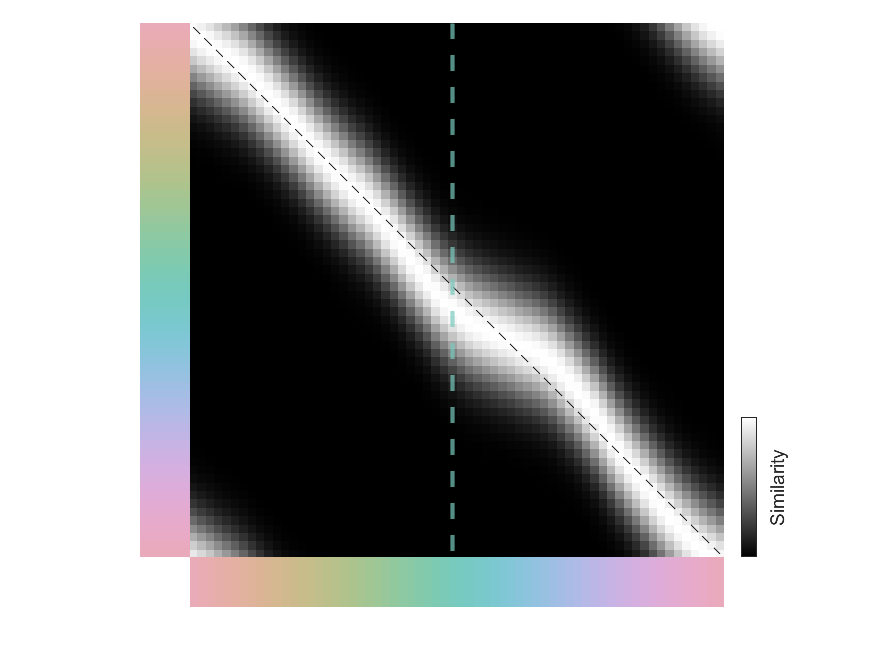
\includegraphics[width=\textwidth,trim={2cm 0.5cm 2 0},clip]{../Figures/working/F3_TCCModel/sm_og_231110-022722.png}
         \label{fig:TCCModel_og_sm}
    \end{subfigure}
    \begin{subfigure}[b]{0.3\textwidth}
         \centering
         \caption{}
         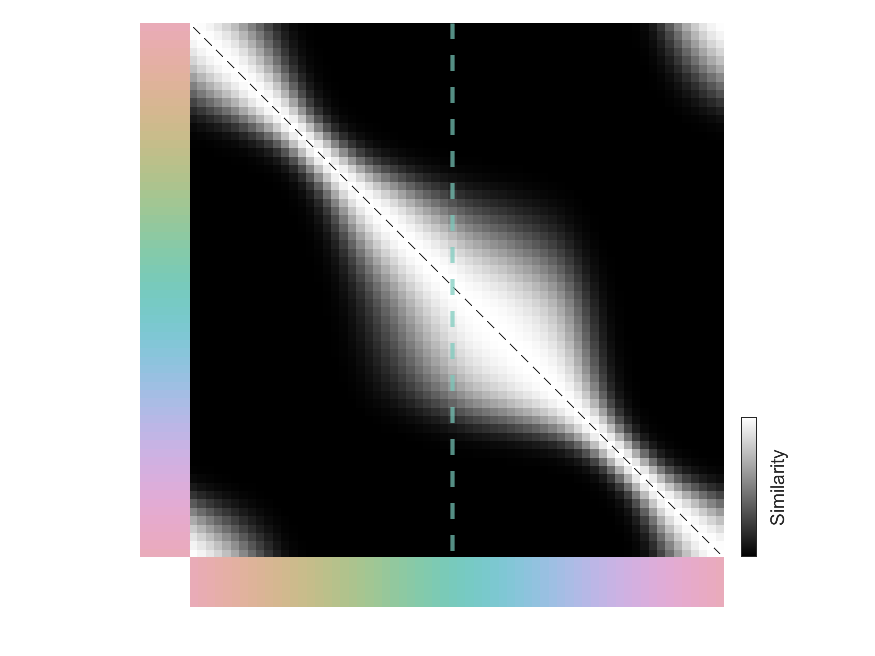
\includegraphics[width=\textwidth,trim={2cm 0.5cm 2 0},clip]{../Figures/working/F3_TCCModel/sm_ssnu_231110-022643.png}
         \label{fig:TCCModel_ssnu_sm}
    \end{subfigure}
    
    \begin{subfigure}[b]{0.3\textwidth}
         \centering
         \caption{}
         \includesvg[pretex=\tiny, width=\textwidth]{../Figures/working/F3_TCCModel/og_SimilarityFunction_231110-022716.svg}
         \label{fig:TCCModel_ssnu_sm}
    \end{subfigure}
    \begin{subfigure}[b]{0.3\textwidth}
         \centering
         \caption{}
         \includesvg[pretex=\tiny, width=\textwidth]{../Figures/working/F3_TCCModel/ssnu_SimilarityFunction_231110-022641.svg}
         \label{fig:TCCModel_ssnu_sm}
    \end{subfigure}

    % \begin{subfigure}[b]{0.45\textwidth}
    %      \centering
    %      \caption{}
    %      \includesvg[pretex=\tiny, width=\textwidth]{../Figures/working/F3_TCCModel/sg_SimilarityFunction_230807-153339.svg}
    %      %\label{fig:JustBias_subset}
    % \end{subfigure}
    % \hfill
    % \begin{subfigure}[b]{0.45\textwidth}
    %      \centering
    %      \caption{}
    %      \includesvg[pretex=\tiny, width=\textwidth]{../Figures/working/F3_TCCModel/ssnu_SimilarityFunction_230731-150035}\llap{\raisebox{3cm}{\includesvg[pretex=\tiny, width=2.5cm]{../Figures/working/F6_ColSpace/combined_TCC-0att_fullremap-workspace_230510_behaviorally-derived-colorspace_everySecond230818-114423.svg}}} 
    %      % h/t: https://tex.stackexchange.com/a/89778/169285 
    %      %\label{fig:JustColSpace_subset}
    % \end{subfigure}
        \caption{\textbf{Distinguishing between different sources of bias using TCC-MAT models: cognitive bias vs. non-uniformity of stimulus space.} Similarity matrices representing different theoretically driven mechanisms can result in the same average bias value. A mixture model cannot distinguish between these different sources, whereas a TCC-MAT model readily can. \ref{fig:TCCModel_og}: an example of how cognitive bias might appear - each row of the matrix is shifted leftwards or rightwards. \ref{fig:TCCModel_ssnu}: an example of how non-uniformity in stimulus space might appear - the similarity between each cue and its neighbors is increased or decreased, resulting in an expansion of the higher similarity region of the matrix symmetrically around the negative diagonal for colors which are more similar to their neighbors than average, and a contraction for colors that are less similar to their neighbors than average. \ref{fig:TCCModel_og_sm}: The values representing the similarity function for cue 20 (the row highlighted in red in \ref{fig:TCCModel_ssnu_sm}), with the circular median shown as a vertical dashed line. \ref{fig:TCCModel_ssnu_sm}: As in \ref{fig:TCCModel_og_sm} but for \ref{fig:TCCModel_ssnu}. Note how the circular median of \emph{both} functions is 25.}
        \label{fig:TCCDemo}
\end{figure}


The colors we used were defined by the International Commission on Illumination (CIE) to be approximately perceptually uniform. 
But it has long been recognized that there may be non-uniformities in the space%{Brainard, 2010 \#4684}
; some have argued that perceptual uniformity may be task-dependent or simply unattainable%{Judd, 1970 \#17915}
. 
One might even suppose that if language influences color perception, as stipulated by the Sapir-Whorf hypothesis, then all color spaces generated by human observers could be shaped by language. 
Could the macaque consensus color categories be attributed not to a true “cognitive” category (\autoref{fig:TCCCartoonA}) but to unrecognized distortions in the presumed uniform space of colors (\autoref{fig:TCCCartoonB})? 

The central difference in the two explanations can be understood by considering the relationship between two neighboring colors. 
For the cognitive-bias account, there is an asymmetry between the colors if there is a category center nearby - the color further from the category center will be more likely mistaken for the color closer to the category center than the other way around. 
Whereas for the non-uniform color space, there is no asymmetry in mismatches between neighboring pairs of colors - if these two colors were more easily confused with eachother than their other neighbors, then on average the response to either would be biased towards a point between them.

To illustrate that the behavioral data could be caused by either a cognitive-bias account or a stimulus-space non-uniformity, we generated two sets of simulated data for our task. 
One simulation used a uniform space with the types of biases that might arise due to categorical encoding, and the other used a distorted color space with two foci of distortion but with explicit biases. 
Both simulations give rise to the same pattern of results when analyzed with a mixture model, and we can generate simulated data such that the pattern qualitatively matches the real behavioral data (\autoref{fig:TCCCartoonA} and \autoref{fig:TCCCartoonB}; compare these simulations with \autoref{fig:CombinedPolar}). 
So, to tease apart the possible underlying causes of the behavioral results, we developed a generative model based on the Target Confusability Competition (TCC) model \citep{schurgin_psychophysical_2020}. 
The key development of our model over that of \cite{schurgin_psychophysical_2020} is that it does not assume the same underlying similarity function for each color - whereas \cite{schurgin_psychophysical_2020} use a similarity function to map distances to similarity scores, we introduce the concept of a similarity matrix, which can be thought of as a unique similarity function per stimulus. 
To recognize this conceptual difference, we refer to these types of models as ``TCC-MAT``.

We consider three versions of this model: a cognitive bias version, a stimulus-space non-uniformity version, and a free-similarity version.
In the cognitive bias TCC-MAT model, the gaussian which defines the similarity function is allowed to float such that the peak need not be at 0, independently for each stimulus (\autoref{fig:TCCModel_og_sm}).
This results in a similarity matrix that is asymmetric about the diagonal.
In the stimulus-space non-uniformity TCC-MAT model, the gaussian is fixed to peak at 0, but the angular distances between each stimulus and the next successive stimulus are allowed to float, again independently for each stimulus (\autoref{fig:TCCModel_ssnu_sm}).
This results in a similarity matrix that is symmetric about the diagonal, but which can bulge out around the diagonal in areas where there is higher than average similarity between neighboring stimuli.
In the most flexible version of TCC-MAT, every cell in the similarity matrix is an independent model parameter.
This allows for a somewhat "model-free" model - it includes no assumptions about the underlying mechanisms that determine the similarity between cue x and choice y, which allows us to assess how well the mechanisms implemented in the more constrained models capture the gross structure of the data.

\begin{figure}
    \centering
    \begin{subfigure}[b]{0.3\textwidth}
         \centering
         \caption{}
         \includesvg[pretex=\tiny, width=\textwidth]{../Figures/working/F4_TCCResults/sm_combined_TCC-FreeSimilarityMatrix-workspace_230214cool_230818-111211.svg}
         \label{fig:SimilarityMatrixCombined_Cool}
    \end{subfigure}
    \hfill
    \begin{subfigure}[b]{0.3\textwidth}
         \centering
         \caption{}
         \includesvg[pretex=\tiny, width=\textwidth]{../Figures/working/F4_TCCResults/sm_combined_TCC-FreeSimilarityMatrix-workspace_230214warm_230818-111210.svg}
         \label{fig:SimilarityMatrixCombined_Warm}
    \end{subfigure}
    \hfill
       \begin{subfigure}[b]{0.3\textwidth}
         \centering
         \caption{}
         \includesvg[pretex=\tiny, width=\textwidth]{../Figures/working/F4_TCCResults/BIC_Combined_230907-051338.svg}
         \label{fig:Combined-ModelFitAnalysis}
    \end{subfigure}
    \caption{\textbf{Free Similarity model fit for combined data from all animals.}
    Similarity between stimulus $s_i$ and stimulus $s_j$, where one is the cue and one is the choice. This is a ``free'' similarity matrix - in that no particular relationship is pre-supposed between any of the stimuli (such as, for example: closer stimuli will be more similar). This figure can be compared to Figure 1D in \cite{schurgin_psychophysical_2020}, except there the rows are circularly shifted so that the the x-axis becomes the relative distance, rather than the absolute value of the stimulus. % should we just plot it the same way at this stage? It doesn't really make a difference here...
    % supplementary figure with alternative plotting method?
    %confidence intervals?!?!?! !!!!!!!!!!!!!!
    } 
    \label{fig:TCCOutput}
\end{figure}

To determine which model better explains the macaque behavioral data, we quantitatively compared the different versions of the model (including also a null-model which does not allow for any biases).

The behavioral data are best explained by the stimulus-space non-uniformity model, as quantified by negative log-likelihood and AIC (\autoref{fig:Combined-ModelFitAnalysis}). 

\begin{figure}
    \centering
    \begin{subfigure}[b]{0.2\textwidth}
         \centering
         \caption{}
         \includesvg[pretex=\tiny, width=\textwidth]{../Figures/working/SI/SI1_IndiMM/210517--211108_Castor_data_fromPreProcessedData_MixMod_polar_230803-000637.svg}
         \label{fig:CastorMM}
    \end{subfigure}
    \hfill
    \begin{subfigure}[b]{0.38\textwidth}
         \centering
         \caption{}
         \includesvg[pretex=\tiny, width=\textwidth]{../Figures/working/F5_CastorCogBias/sm_18_230731-150331.svg}
         \label{fig:Castor-FreeSimilarity}
    \end{subfigure}
    \hfill
       \begin{subfigure}[b]{0.38\textwidth}
         \centering
         \caption{}
         \includesvg[pretex=\tiny, width=\textwidth]{../Figures/working/F5_CastorCogBias/BIC_Castor_230907-052020.svg}         \label{fig:fig:Castor-ModelFitAnalysis}
    \end{subfigure}
    \caption{\textbf{Lorem}
    Ipsum}
    \label{fig:IndiDataCogBias}
\end{figure}

\paragraph{Idiosyncratic categories in individual animals}
But does the TCC-c model have sufficient sensitivity to discover a cognitive bias should one exist? 
The data for individual animals shows that it does. 
By mixture-model analysis, one animal showed not only the two consensus choice biases for “warm” and “cool” but also a strong choice bias for pea green (\autoref{fig:CastorMM}). 
The free similarity matrix for the data from this animal shows an asymmetry about the diagonal corresponding to this color (\autoref{fig:Castor-FreeSimilarity}), providing the hallmark of a cognitive color bias that is confirmed by negative log-likelihood and AIC quantification (\autoref{fig:fig:Castor-ModelFitAnalysis}).


\begin{figure}
    \centering
    \begin{subfigure}[b]{0.3\textwidth}
         \centering
         \caption{}
         \includesvg[pretex=\tiny, width=\textwidth]{../Figures/working/F6_ColSpace/colorspace_everySecond230818-114428.svg}
         \label{fig:CIELUV}
    \end{subfigure}
    \hfill
    \begin{subfigure}[b]{0.3\textwidth}
         \centering
         \caption{}
         \includesvg[pretex=\tiny, width=\textwidth]{../Figures/working/F6_ColSpace/combined_TCC-0att_fullremap-workspace_230510_behaviorally-derived-colorspace_everySecond230818-114423.svg}
         \label{fig:MACBEHspace}
    \end{subfigure}
    \hfill
    \begin{subfigure}[b]{0.3\textwidth}
         \centering
         \caption{}
         \includesvg[pretex=\tiny, width=\textwidth]{../Figures/working/F6_ColSpace/newEqualSampling230818-170747.svg}
         \label{fig:UniformStimsInCIELUV}
    \end{subfigure}
           \caption{\textbf{A behaviorally-derived colorspace.} Stimuli in CIELUV. Stimuli in behaviorally-derived space. Stimuli sampled in behaviorally-derived space, projected back into CIELUV.}
        \label{fig:MACBEHcolorspace}
    
\end{figure}


\paragraph{A perceptually uniform color space unconfounded by language}

The behavioral data in macaques provide a rare opportunity to reconstruct a perceptually uniform color space unconfounded by language. 
We computed, empirically, a transformed colorspace such that the macaques would, on average, show no choice bias.
When colors evenly sampled from the purportedly uniform CIELu*v* space (\autoref{fig:CIELUV}) are plotted within this macaque-derived uniform color space, colors around the teal part of the space collect, and to a lesser extent, so do colors in the salmon-peach part of the space (\autoref{fig:MACBEHspace}). 

\paragraph{Categorical intrusion in the creation of colorspaces}

The non-uniformities in the CIE CIELu*v* space implied by these results raise a question about their origin. 
Given color categories can be learned, as evident in at least one macaque in our study (\autoref{fig:Castor-FreeSimilarity}, and \autoref{fig:SimilarityMatrixIndividual}) and two macaques in another study \citep{panichello_error-correcting_2019}, coupled with the likely possibility that this learning reflects colors of environmental or behavioral relevance, we wondered whether the distortions in the presumed uniform color space could be attributed to the warm and cool color categories manifest in apparently all human cultures \citep{gibson_color_2017} and hypothesized to be caused by the non-arbitrary color statistics of objects and backgrounds \citep{rosenthal_color_2018}
— objects are more likely to be warm-colored and backgrounds, cool-colored. 
To test this idea, we ran a simulation in which the macaque uniform color space was used in a color-matching task by an agent with cognitive biases for warm and cool colors defined by the average colors of objects and backgrounds. 
The resulting similarity space of colors shows a distortion — a non-uniformity — that corresponds to the distortion inferred from the macaque behavioral data. 
These results provide a plausible mechanism by which the distortions in the color space arise and suggest that all color spaces made by human observers are inexorably impacted by the universally behaviorally relevant categories of warm and cool. 

% Left to incorporate: 
% different colorspaces, optimised for different tasks, could exist at different levels of the visual hierarchy. 

% Saturation bias

% 4-Alternative Forced Choice: Human participants

